\documentclass{article}
\usepackage{hyperref}
\usepackage{amsmath}
\usepackage{graphicx}
\graphicspath{~/pandoc-test/Stat159/stat159-fall2016-project3}
\usepackage{Sweave}
\begin{document}

\title{Report}
\author{Eranda Bregasi, Leanne Lee, Jamie Stankiewiz}
\date{12/2/16}
\maketitle

\Sconcordance{concordance:report.tex:report.Rnw:%
1 2 1 1 0 9 1 1 8 1 4 19 0 1 2 14 1 1 2 7 0 1 2 2 1}





\section{Abstract}

  This project focuses on providing our client from the biotech industry with the most qualified schools who fulfill their criterias of recruitment.  To determine the best scshools for our client, we need to set a bar on what determines a ''top school``.  To achieve this, we will focus on the use of College ScoreCard dataset.  To determine which schools contain the highest achieving biotech students, we have set our dependent variable to be earnings after graduation.  We will then look at how our other independent variables influence the earnings. 

\section{Introduction}

  The purpose of this research is to find the schools that contain high achieving students in the fields of Science, Technology, Engineering and Mathematics (STEM).   
In order to determine the top schools in the country, we first have to set restrictions of certain categories that describe the quality of a school.
These ``qualities'' encompass standardized test data such as the school's average SAT math and ACT scores as well as the school's admission rate.  Higher average test scores imply that the students at that school are smarter than students of schools with lower average test scores.  Schools with lower admission rate imply that the school is much harder to get into, opposed to a school with a higher admission rate.
To achieve this, we will look at the data of the schools and partition the schools such that we only have the ``top'' schools in the country.  
After our data cleaning process, we focus particularly on these top schools that remain to figure out the percentage of students who received a 4 year degree in STEM fields.  
After this step, we can narrow our search to look for specific criterion of interest.  For example, we can look to see if students who received pell-grant with high SAT math/ACT scores attend more selective schools, which have a low admission rate and higher graduation rate.  This directly affects our dependent variable of earnings, since it leads to higher earnings.  
For the completion of this project and to have an effective and accurate comparison of our data, we chose to use three different kinds of regression models that we learned throughout the semester. 
We used multiple linear regression, ridge regression, and random forest to fit our data against different tiers of earnings.  The reason we chose these regressions are because of the collinearities.  Our predictors include the SAT math and ACT scores, the admission, graduation rate after the 4 years of attendance in a higher institution and pell grant recipients.  Finally our dependent variable consists of earnings 10 years after graduation in different tiers.  


\section{Dataset}

  We use the dataset \emph{CollegeScore Card} from \url{https://collegescorecard.ed.gov/data/}. In \emph{data-subsetting.R}, we subset 34 columns that we need for the project. We carefully examined each predictors and see which predictors fit our needs to increase the performance in analysis.  In \emph{data-cleaning.R},  there's a lot of null data and privacy suppressed data so we have to delete those rows and replace some with N/A. After cleaning the data we put them in different csv files. In the \emph{pre-processing.R} we select schools with top SAT math and ACT scores that are at least one standard deviation above average, and then we turn those columns that we need into numerics from factors. We decided on 5 predictors and 1 dependent variable out of the 34 options. Finally, we export the clean dataset into a \emph{topschool.csv}.

\begin{Schunk}
\begin{Soutput}
 [1] "X"                    "INSTNM"               "CITY"                
 [4] "STABBR"               "ZIP"                  "ADM_RATE"            
 [7] "SATMT75"              "ACTMT75"              "COMP_ORIG_YR4_RT"    
[10] "PCIP11"               "PCIP14"               "PCIP15"              
[13] "PCIP26"               "PCIP27"               "PCIP29"              
[16] "PCIP40"               "PCIP41"               "C150_4"              
[19] "MN_EARN_WNE_INC1_P10" "MN_EARN_WNE_INC2_P10" "MN_EARN_WNE_INC3_P10"
[22] "PCT90_EARN_WNE_P6"    "ICLEVEL"             
\end{Soutput}
\end{Schunk}
We have decided it was useful to keep descriptive categories such as 
\begin{Schunk}
\begin{Soutput}
[1] "X"      "INSTNM" "CITY"   "STABBR"
\end{Soutput}
\end{Schunk}

which give the institution name, city, state, and zip code respectively.  In deciding which categories will give a college certain desirable characteristics for our client, we broke the factors into 3 parts:

\begin{enumerate}
\item Pre-Admission: Data that describe how hard it is to get into a certain college
\item In-school: Data to tell us how many students graduate from each school and department of interest
\item Post-graduation: Data that will describe how much students make after graduating
\end{enumerate}


Among the quantitative variables, pre-admission data includes the school's 75th percentile of the SAT math and ACT scores:
\begin{Schunk}
\begin{Soutput}
[1] "SATMT75" "ACTMT75"
\end{Soutput}
\end{Schunk}
as well as the school's average admission rate: 
\begin{Schunk}
\begin{Soutput}
[1] "ADM_RATE"
\end{Soutput}
\end{Schunk}
In-school data includes the school's graduation rate 
\begin{Schunk}
\begin{Soutput}
[1] "COMP_ORIG_YR4_RT"
\end{Soutput}
\end{Schunk}
as well as the "percentage of degrees awarded in" 8 specific programs named, 
\begin{Schunk}
\begin{Soutput}
[1] "PCIP11" "PCIP14" "PCIP15" "PCIP26" "PCIP27" "PCIP29" "PCIP40" "PCIP41"
\end{Soutput}
\end{Schunk}
which respectively stand for:
\begin{center}
\begin{flushleft}
PCIP11 = computer and information sciences and support services \newline
PCIP14 = engineering \newline
PCIP15 = engineering technologies and engineering related fields \newline
PCIP26 = biological and biomedical sciences \newline
PCIP27 = mathematics and statistics \newline
PCIP29 = military technologies and applied sciences \newline
PCIP40 = physical sciences \newline
PCIP41 = science technologies/technicians \newline
\end{flushleft}
\end{center}
  These variables will help us to determine the quality of the school, and the size of each program.  Post-graduation data includes the ``mean earnings of students working and not enrolled 10 years after entry in" 3 different categorical earnings denoted:  

\begin{Schunk}
\begin{Soutput}
[1] "MN_EARN_WNE_INC1_P10" "MN_EARN_WNE_INC2_P10" "MN_EARN_WNE_INC3_P10"
\end{Soutput}
\end{Schunk}
\begin{flushleft}
MN\_EARN\_WNE\_INC1\_P10 = ``lowest income tercile \$0-\$30,000" - low tier \newline
MN\_EARN\_WNE\_INC2\_P10 = ``middle income tercile \$30,001-\$75,000" - middle tier \newline
MN\_EARN\_WNE\_INC3\_P10 = ``highest income tercile \$75,001  " - top tier \newline
\end{flushleft}
These categories will be used in our regression-models to help us determine the top schools as well as the visualizations created.

  Once we have properly subsetted our dataset, it was necessary to clean it in order to be  properly used.  In particular, all of the PCIP columns that contained the value 0 was replaced by NA.  We then needed to take out only the schools that were a 4 year institution, 
\begin{Schunk}
\begin{Soutput}
[1] "ICLEVEL"
\end{Soutput}
\end{Schunk}
in this dataset, this column is categorical: 
  \begin{flushleft}
  1 = 4-year institution \newline
  2 = 2-year institution \newline
  3 = less than 2-year institution \newline
  \end{flushleft}
  For our analysis, the only schools our client should be interested in are top 4-year institutions.  So we subsetted our data set appropriately.

\section{Methodology}

  We used regression analyses in this project because we wanted to determine if average earnings after graduation is dependent on the school's level of difficulty.  
We picked 3 different regression analyses to find out which model fits our data the best.  
The 3 regressions of choice are: multiple linear regression, ridge regression and random forest.   
In our regressions, the independent variables are: SAT  math \& ACT scores (SATMT75 \& ACTMT75), admission rate (ADM\_RATE) and graduation rate (COMP\_ORIG\_YR4\_RT).  These factors will help us to predict our 
response variable, highest earnings 10 after graduation (MN\_EARN\_WNE\_INC3\_P10).  We have also gone through to analyze the the same regressions with the response variable being the other 2 categories of middle and lowest earnings (MN\_EARN\_WNE\_INC2\_P10, MN\_EARN\_WNE\_INC1\_P10).  

  We used multiple linear regression to provide a basic analysis to look at how the predictor variables independently affect the response variable.  
While multiple linear regression is a good start, it is most likely that the predictor variables are not independent.  For that case, ridge regression is a better model.  This is because our predictor variables are collinear.  
After comparing the results between multiple linear regression and ridge regression, we use random forest to predict the future earnings of high achieving students.  The random forest method is a good fit for our case because it is more robust to multi-collinearities. 


\subsection{Overview of Regression Models}

\textbf{Multiple Linear Regression} \newline
The goal of multiple linear regression is to see how our response variable changes when it is dependent on other variables.  These variables are assumed to be invariant from each other so we can look at how the response variables changes when only one predictor variables changes at a time, keeping the other variables constant.  The multiple linear regression model is given by:

$$\hat Y = \hat \beta_0 + \hat \beta_1 X_1 + \hat \beta_2 X_2 + \dots + \hat \beta_p X_p + \hat \epsilon$$

Where the betas are the effective increase in Y with a unit increase in $X_i$, holding the other variables fixed.  
The goals is to find the estimates of $\beta_i$ by using $\hat \beta_i$ and use the ANOVA analysis to determine which variables are significant to predicting the response variable.
\newline
\newline
\textbf{Ridge Regression}\newline
Ridge regression is similar to OLS with the coefficients estimated by minimizing a slightly different quantity.  By minimizing RSS, we can find the coefficient estimates that fit the data well. 

$$\sum_{i=1}^{n}(y_i-\beta_0-\sum_{j=1}^{p}\beta_jx_{ij})^2+\lambda\sum_{j=1}^{p}\beta_j^2 = RSS + \lambda\sum_{j=1}^{p}\beta_j^{2}$$ 

However, the shrinkage penalty is that $\lambda\sum_{j=1}^{p}\beta_j^{2}$ is small when $\beta$ are close to zero. Ridge regression will produce a different set of coefficient estimates for each value of $\lambda$ .
\newline
\newline
\textbf{Random Forest}\newline
Random forest is another regression method that constructs many ''decision trees`` on the training data, more of a machine learning bootstrap.  Decision trees partition the data one variable at a time to decrease the residual sum of squares. 

Random forest also outputs 2 additional measurements:
\begin{itemize}
\item Variable importance: this is essence, ranks the variables of greatest importance (done by looking at how much the error value changes when you only change the independent variable, keeping the other variables constant)
\item Neighbor proximity: this is used to determine the ''structure`` of the data
\end{itemize}

$$\hat y =  \sum_{i=1}^{n} \left(\frac{1}{m} \sum_{i=1}^{m} (W_j(x_i,x')\right)y_i$$

Here, W is a weight function that takes the new point $x'$ and weights it relative to a neighbor point, $x_i$.  Altogether, these predict the new $\hat y$.



\section{Analysis}

\textbf{Multiple Linear Regression}\newline
% latex table generated in R 3.3.1 by xtable 1.8-2 package
% Thu Dec 01 21:59:47 2016
\begin{table}[ht]
\centering
\begin{tabular}{r}
  \hline
R\_squared\_summary \\ 
  \hline
0.6029138 \\ 
  0.6168404 \\ 
  0.5795355 \\ 
   \hline
\end{tabular}
\end{table}\newline
  The chart above shows the r-squared when comparing our predictors against earning after graduation in three tiers. The r-squared in this class is similar for top and middle tiers.  However, if we compared the r-squared with just top and bottom tiers, we can see that top tier of 
\begin{Schunk}
\begin{Sinput}
> TopLMsum
\end{Sinput}
\begin{Soutput}
[1] 0.6029138
\end{Soutput}
\end{Schunk}
is performing better than 
\begin{Schunk}
\begin{Sinput}
> LowLMsum
\end{Sinput}
\begin{Soutput}
[1] 0.5795355
\end{Soutput}
\end{Schunk}


% latex table generated in R 3.3.1 by xtable 1.8-2 package
% Thu Dec 01 21:59:47 2016
\begin{table}[ht]
\centering
\begin{tabular}{r}
  \hline
MSE\_summary \\ 
  \hline
0.3939347 \\ 
  0.3801186 \\ 
  0.4171275 \\ 
   \hline
\end{tabular}
\end{table}Again, this MSE chart also have values that are similar within different tiers. However, low tier is still performing worse than the top and middle tiers. Since low tier has the highest MSE of 
\begin{Schunk}
\begin{Sinput}
> LowMSE
\end{Sinput}
\begin{Soutput}
[1] 0.4171275
\end{Soutput}
\end{Schunk}
it has more errors from the data than the other tiers. 


The reason that top tier and middle tier are very close to each other is because of the large range of the middle tier. The middle tier encorperates the students' earnings after graduation, this range is between \$30,001-\$75,000. Many STEM and non-STEM students can fall into this bracket because this is the average earning after graduation for most schools in the United States.  
\newline

The following data are the coefficients of each earning bracket from the multuple linear regression:
\begin{Schunk}
\begin{Sinput}
> TopCoef
\end{Sinput}
\begin{Soutput}
          (Intercept)               SATMT75               ACTMT75 
        -4.646350e-16          2.517286e-01          3.705993e-01 
             ADM_RATE PELL_COMP_ORIG_YR6_RT      COMP_ORIG_YR4_RT 
        -1.391154e-01         -3.840951e-01          3.259766e-01 
\end{Soutput}
\begin{Sinput}
> MidCoef
\end{Sinput}
\begin{Soutput}
          (Intercept)               SATMT75               ACTMT75 
        -6.646505e-16          2.953424e-01          4.062549e-01 
             ADM_RATE PELL_COMP_ORIG_YR6_RT      COMP_ORIG_YR4_RT 
        -1.238959e-01         -2.978452e-01          2.041115e-01 
\end{Soutput}
\begin{Sinput}
> LowCoef
\end{Sinput}
\begin{Soutput}
          (Intercept)               SATMT75               ACTMT75 
        -6.021958e-16          2.537037e-01          3.882197e-01 
             ADM_RATE PELL_COMP_ORIG_YR6_RT      COMP_ORIG_YR4_RT 
        -1.214981e-01         -2.095447e-01          2.178538e-01 
\end{Soutput}
\end{Schunk}

First, let look at the coefficient in the top tier.  We can see that there is a positive relationship effect for SAT math, ACT and graduation rate against the top tier of earning.  For every standard deviation of SAT math score increases, there is an increase in 
\begin{Schunk}
\begin{Sinput}
> TopCoef['SATMT75']
\end{Sinput}
\begin{Soutput}
  SATMT75 
0.2517286 
\end{Soutput}
\end{Schunk}
standard deviation increase in top tier earning. From the coefficients, we can also see that the admission rate and pell grant recipient have a negative relationship against top tier earnings.  For every standard deviation (of admission rate) that increases, there is a decrease in top tier earnings.  The negative relationship makes sense because for schools with a higher admission rate, we expect it to result in lower earnings.  Since we are only looking at students who perform well in SAT math and ACT scores, these students are more likely be admitted into more selective schools, implying a lower admission rate.  When we look at the negative relationship for the pell grant recipient, we also see a negative relationship.  For every standard deviation increase in pell grant recipient, there is a decrease in earnings. 
When we compare the coefficient in the low tier, we can see that SAT math and ACT score still makes a positive effect on earning. However, there is a slight decrease in pell grant and graduation rate.  It shows that there is a less increase in earnings for each standard deviation of increase in graduation rate. 
\newline
\newline

\textbf{Ridge Regression}\newline
% latex table generated in R 3.3.1 by xtable 1.8-2 package
% Thu Dec 01 21:59:47 2016
\begin{table}[ht]
\centering
\begin{tabular}{rr}
  \hline
 & MSE \\ 
  \hline
Top Tier Earnings & 0.3974380 \\ 
  Middle Tier Earnings & 0.3873009 \\ 
  Lower Tier Earnings & 0.4223115 \\ 
   \hline
\end{tabular}
\end{table}\newline

  Since ridge regression does not have r-squared values, we can compare the MSE values from the ridge regression with the multiple linear regression.  We can see that the MSE values from ridge regression are fairly close to the MSE values from multiple linear regression. 

  The following data are the coefficients of each tier earning generated from the ridge regression.  The order of the tables are as follows: Top Tier Earnings, Middle Tier Earnings, Lowest Tier Earnings \newline
% latex table generated in R 3.3.1 by xtable 1.8-2 package
% Thu Dec 01 21:59:49 2016
\begin{table}[ht]
\centering
\begin{tabular}{rr}
  \hline
 & x \\ 
  \hline
Intercept & 0.0000000 \\ 
  SATMT75 & 0.2530749 \\ 
  ACTMT75 & 0.3483071 \\ 
  ADM\_RATE & -0.1614524 \\ 
  COMP\_ORIG\_YR4\_RT & 0.2500293 \\ 
  PELL\_COMP\_ORIG\_YR6\_RT & -0.3077931 \\ 
   \hline
\end{tabular}
\end{table}% latex table generated in R 3.3.1 by xtable 1.8-2 package
% Thu Dec 01 21:59:49 2016
\begin{table}[ht]
\centering
\begin{tabular}{rr}
  \hline
 & x \\ 
  \hline
Intercept & 0.00 \\ 
  SATMT75 & 0.29 \\ 
  ACTMT75 & 0.36 \\ 
  ADM\_RATE & -0.16 \\ 
  COMP\_ORIG\_YR4\_RT & 0.14 \\ 
  PELL\_COMP\_ORIG\_YR6\_RT & -0.22 \\ 
   \hline
\end{tabular}
\end{table}% latex table generated in R 3.3.1 by xtable 1.8-2 package
% Thu Dec 01 21:59:49 2016
\begin{table}[ht]
\centering
\begin{tabular}{rr}
  \hline
 & x \\ 
  \hline
Intercept & 0.00 \\ 
  SATMT75 & 0.25 \\ 
  ACTMT75 & 0.33 \\ 
  ADM\_RATE & -0.16 \\ 
  COMP\_ORIG\_YR4\_RT & 0.15 \\ 
  PELL\_COMP\_ORIG\_YR6\_RT & -0.13 \\ 
   \hline
\end{tabular}
\end{table}\newline
  When we compare the ridge coefficients with multiple linear regression coefficients, it shows a larger positive relationship between SAT math/ACT scores and earnings.  For every standard deviation increase in SAT math/ACT scores, there is a higher increase in standard deviation of earnings. The ridge regression coefficient also shows a negative relationship between admission rate and pell grant recipient against high earnings.
\newline
\newline

\textbf{Random Forest} \newline
  After comparing the coefficients, r-squared and MSE values from multiple linear regression and ridge regression, we used random forest to predict earnings. 

% latex table generated in R 3.3.1 by xtable 1.8-2 package
% Thu Dec 01 21:59:49 2016
\begin{table}[ht]
\centering
\begin{tabular}{rr}
  \hline
 & IncNodePurity \\ 
  \hline
SATMT75 & 20.1190023 \\ 
  ACTMT75 & 19.6249217 \\ 
  ADM\_RATE & 23.9492907 \\ 
  COMP\_ORIG\_YR4\_RT & 13.4489085 \\ 
  PELL\_COMP\_ORIG\_YR6\_RT & 11.8486366 \\ 
   \hline
\end{tabular}
\end{table}
  In random forest regression, we can look at the importance of the model.  It consists of ``IncNodePurity", which is the average cummulative reduction in node impurity due to splits by a variable over the trees. It is also the mean decrease in MSE.  From the variance importance, we can see that the main positive relationships are from SAT math and ACT scores, concluding an existing positive correlation with mean earnings.  From the random forest model, we can choose the best features that represent our data.  Also, the more selective schools that have a lower admission rate also play an important factor with mean earnings. 


\section{Results}

\textbf{Multiple Linear Regression}\newline

\begin{figure}[h!]
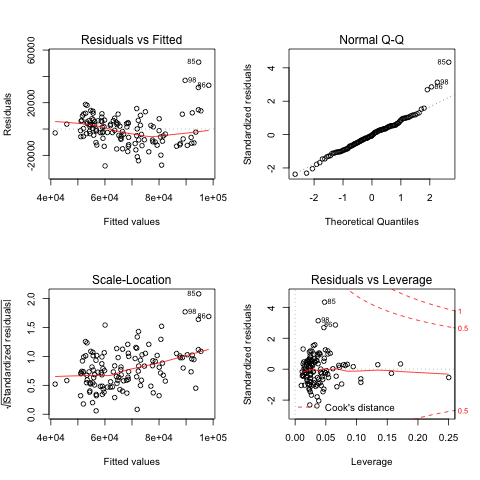
\includegraphics{../images/lm_top.png}
\end{figure}


\textbf{Ridge Regression} \newline
\begin{figure}[h!]
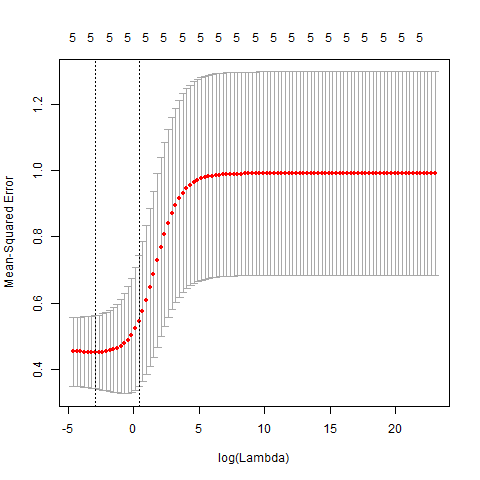
\includegraphics{../images/ridgeCV_top.png}
\end{figure}


\textbf{Random Forest}\newline
\begin{figure}[h!]
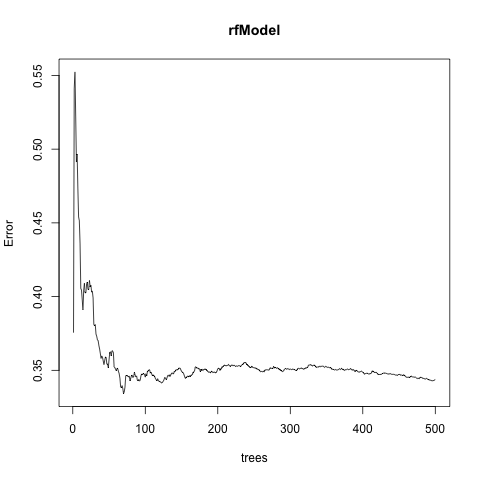
\includegraphics{../images/rf_top.png}
\end{figure}
The plot shows that the error become more stable after 50 decision trees.



There is a positive relationship for high graduation rate, SAT math and ACT scores, which leads to an increase in mean earnings after graduation.  There is also a negative relationship for lower admission rate and pell grant recipients.  Schools that are more selective accept less students; so from our findings, an increase in admission rate would harm the mean earnings.  In addition, pell grant recipients usually come from below average family backgrounds, which lead to less earnings after graduation. 


\begin{figure}[h!]
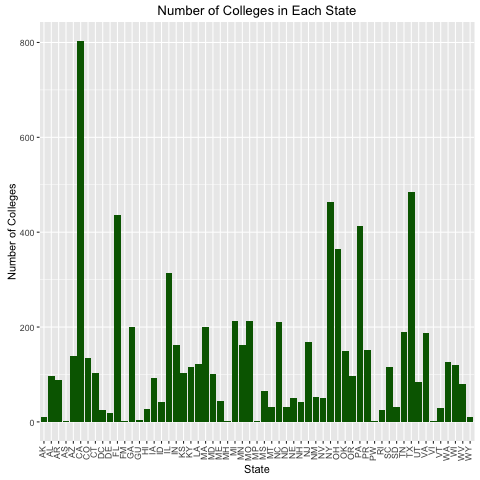
\includegraphics{../images/college-frequency.png}
\end{figure}
In this plot, we can see most top schools come from California. 


Then, we determine the biggest programs from these top schools according to the major. 
Biology 
\begin{figure}[h!]
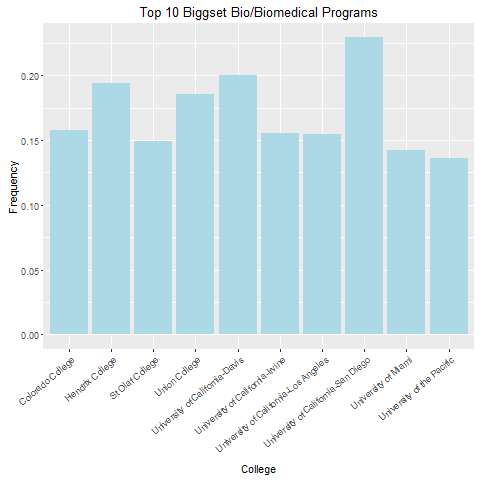
\includegraphics{../images/biggestBio.png}
\end{figure}


Computer Science
\begin{figure}[h!]
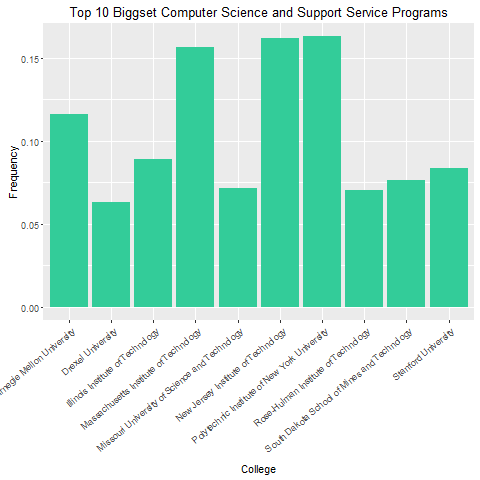
\includegraphics{../images/biggestCS.png}
\end{figure}


Engineering
\begin{figure}[h!]
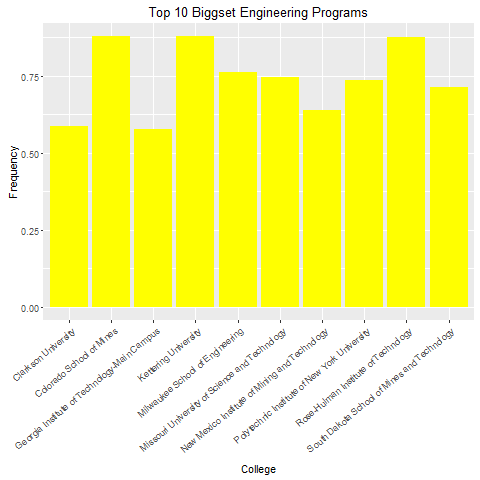
\includegraphics{../images/biggestEngineering.png}
\end{figure}


Math/Statistics
\begin{figure}[h!]
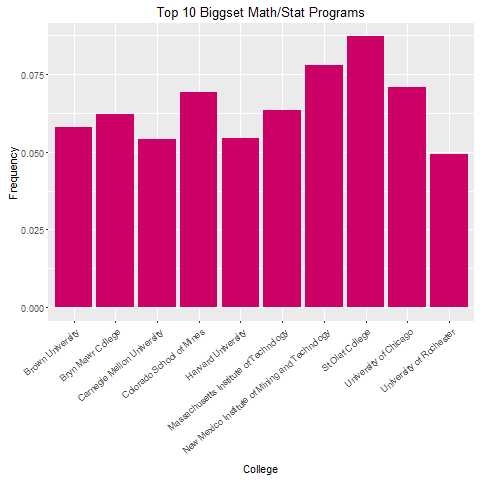
\includegraphics{../images/biggestMathStat.png}
\end{figure}


Technicians
\begin{figure}[h!]
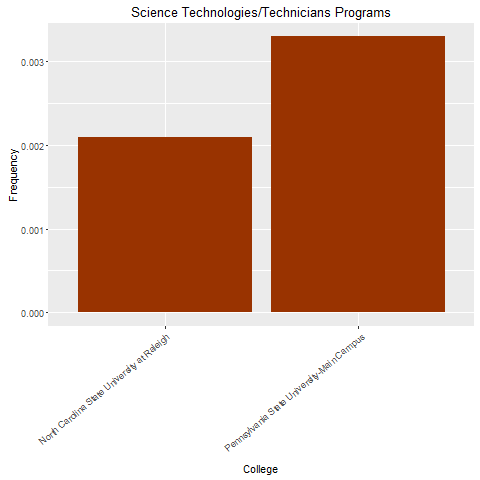
\includegraphics{../images/biggestTechnicians.png}
\end{figure}


Physical Science 
\begin{figure}[h!]
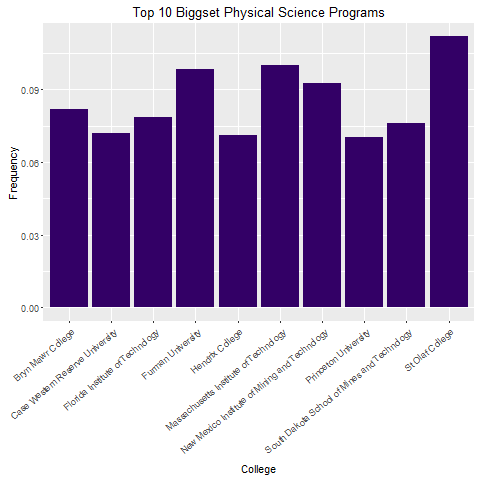
\includegraphics{../images/biggestPhysical.png}
\end{figure}


A tech company can easily find which school produces high achieving students with a large program according to the major. 

\section{Conclusions}


\end{document}
